% Documentation proposal, snapshot 14 October 2026; no new hardware validation.
% WBR advisor progress report -- evidence snapshot 2026-10-13.
% Build: latexmk -xelatex main.tex   (see README.md)
% Content sources and number provenance: SOURCES.md.
% Historical Pi measurements are labeled MEASURED; calculations, assumptions,
% published comparisons, plans and OPEN qualification remain distinct.
\documentclass[aspectratio=169,12pt,t]{beamer}

% Speaker notes: uncomment ONE line to see them.
% \setbeameroption{show notes on second screen=right}  % dual-screen (pdfpc)
% \setbeameroption{show only notes}                     % notes handout

\usetheme[progressbar=none, sectionpage=none]{moloch}
% A 208 x 117 mm canvas retains 16:9 and the actual 12pt class fonts.
% Long owner-approved sentences fit without frame scaling or reduced fonts.
\geometry{paperwidth=208mm,paperheight=117mm}

% ---------- fonts ----------
\usepackage{fontspec}
\setsansfont{Avenir Next}[BoldFont={Avenir Next Demi Bold}]
\setmonofont{Menlo}[Scale=1.0]
\newcommand{\captiontype}{\small}

% ---------- palette ----------
\definecolor{navy}{HTML}{1F3A5F}
\definecolor{teal}{HTML}{2A9D8F}
\definecolor{fault}{HTML}{E76F51}
\definecolor{paper}{HTML}{FAFAF7}
\definecolor{ink}{HTML}{22262B}
\definecolor{muted}{HTML}{6B7280}
\definecolor{rule}{HTML}{D6D9DE}

\setbeamercolor{normal text}{fg=ink, bg=paper}
\setbeamercolor{frametitle}{fg=paper, bg=navy}
\setbeamercolor{progress bar}{fg=teal, bg=rule}
\setbeamercolor{alerted text}{fg=fault}
\setbeamercolor{example text}{fg=teal}
\setbeamercolor{structure}{fg=navy}
\setbeamercolor{title separator}{fg=teal}
\setbeamercolor{footline}{fg=muted}
% Beamer otherwise inherits the fault/alert color for in-slide citations.
\setbeamercolor{bibliography entry author}{fg=navy}
\setbeamercolor{bibliography entry title}{fg=ink}
\setbeamercolor{bibliography entry location}{fg=muted}
\setbeamercolor{bibliography entry note}{fg=muted}
\setbeamercolor{block title}{fg=paper, bg=navy}
\setbeamercolor{block body}{bg=navy!6}
\setbeamerfont{frametitle}{size=\large, series=\bfseries}
\setbeamertemplate{frametitle}{\nointerlineskip\begin{beamercolorbox}[wd=\paperwidth,sep=2mm,leftskip=4mm]{frametitle}\usebeamerfont{frametitle}\insertframetitle\strut\end{beamercolorbox}}
\setbeamertemplate{itemize items}{\color{teal}\rule[0.25ex]{0.45em}{0.45em}}
\setbeamertemplate{bibliography item}[text]
\setbeamertemplate{page number in head/foot}[totalframenumber]
\hypersetup{colorlinks=true, linkcolor=navy, urlcolor=navy, citecolor=navy}
% Keep the appendix bookmark free of Beamer translation commands.
\pdfstringdefDisableCommands{\def\translate#1{#1}}

\setbeamertemplate{itemize subitem}{\color{muted}--}

% ---------- packages ----------
\usepackage{tikz}
\usetikzlibrary{arrows.meta, positioning, automata, calc, shapes.geometric, fit, backgrounds, decorations.pathreplacing}
\usepackage{booktabs}
\usepackage{array}
\newcolumntype{L}[1]{>{\raggedright\arraybackslash}p{#1}}
\usepackage{amsmath}
\usepackage{siunitx}
\sisetup{detect-all}

% ---------- helpers ----------
\newcommand{\muted}[1]{{\color{muted}#1}}

% \slideimg[<max height>]{<width>}{<V-id>}{<caption for placeholder>}
% Shows images/<V-id>.jpg or .png if present, otherwise a labelled gray box of the same size.
\newcommand{\slideimg}[4][0.64\textheight]{%
  \IfFileExists{images/#3.jpg}{%
    \includegraphics[width=#2, height=#1, keepaspectratio]{images/#3.jpg}%
  }{\IfFileExists{images/#3.png}{%
    \includegraphics[width=#2, height=#1, keepaspectratio]{images/#3.png}%
  }{%
    \begin{tikzpicture}
      \node[draw=rule, fill=black!6, rounded corners=2pt, minimum width=\dimexpr#2-1pt\relax, outer sep=0pt,
            minimum height=#1, align=center, text width=\dimexpr#2-8mm\relax, font=\small, text=muted]
        {\textbf{#3}\\[2pt]#4\\[2pt]\small Illustration pending};
    \end{tikzpicture}%
  }}%
}

\tikzset{
  box/.style={draw=navy, fill=white, rounded corners=2pt, align=center, font=\small,
              minimum height=7mm, inner sep=3pt},
  flow/.style={-{Stealth[length=2mm]}, thick, color=navy},
  faultflow/.style={-{Stealth[length=2mm]}, thick, color=fault},
  lbl/.style={font=\small, color=ink, fill=paper, inner sep=1pt},
}

% Only the page number appears in the footer.
\setbeamerfont{footline}{size=\small}
\setbeamertemplate{footline}{\hbox{\begin{beamercolorbox}[wd=\paperwidth,ht=4mm,dp=1mm,rightskip=6mm]{footline}\hfill\insertframenumber/\inserttotalframenumber\end{beamercolorbox}}}
\AtBeginSection{\begin{frame}[c]\centering{\Huge\bfseries\color{navy}\thesection. \insertsectionhead\par}\end{frame}}
\setbeamertemplate{navigation symbols}{}
\setbeamersize{text margin left=6mm,text margin right=6mm}
\setlength{\tabcolsep}{4pt}
\renewcommand{\arraystretch}{1.02}
\title{WBR Perception: Progress Report}
\subtitle{Known baseline before camera adaptation}
\author{}
\institute{}
\date{13 October 2026}


\newcounter{slidefigure}
\newcommand{\figcap}[1]{\par\smallskip{\centering\captiontype\color{muted}\refstepcounter{slidefigure}Figure \theslidefigure: #1\par}}
\newcommand{\figagain}[1]{\par\smallskip{\centering\captiontype\color{muted}Figure~\ref{fig:#1}: \csuse{caption#1}\par}}
\setbeamerfont{bibliography entry author}{size=\normalsize}
\setbeamerfont{bibliography entry title}{size=\normalsize}
\setbeamerfont{bibliography entry location}{size=\normalsize}
\setbeamerfont{bibliography entry note}{size=\normalsize}
\setlength{\emergencystretch}{2em}
\setbeamerfont{normal text}{size=\normalsize}
\setbeamerfont{itemize/enumerate body}{size=\normalsize}
\setbeamerfont{itemize/enumerate subbody}{size=\normalsize}
\linespread{1.12}
\AtBeginDocument{\setlength{\leftmargini}{1.1em}\setlength{\leftmarginii}{1.2em}\setlength{\labelsep}{.35em}}
\newcommand{\namedcap}[2]{\figcap{#2}}
% Apply spacing after Beamer has created each list (including nested lists).
\usepackage{etoolbox}
\makeatletter
\apptocmd{\itemize}{\ifnum\@itemdepth=1\setlength{\itemsep}{.55em}\else\setlength{\itemsep}{.25em}\fi\setlength{\parsep}{0pt}\setlength{\parskip}{0pt}\setlength{\topsep}{0pt}}{}{}
\makeatother
\newsavebox{\figurebox}
\newcommand{\fig}[3][.48\textheight]{%
  \ifcsdef{diagram#2}{\sbox{\figurebox}{\csuse{diagram#2}}}{%
    \sbox{\figurebox}{\includegraphics[width=\linewidth,height=#1,keepaspectratio]{images/#2.jpg}}}%
  \par\centering\begin{minipage}{\wd\figurebox}\centering
  \usebox{\figurebox}%
  \ifcsdef{assetcaption#2}{\csuse{assetcaption#2}}{%
    \csgdef{assetcaption#2}{\repeatassetcap{#2}}%
    \csgdef{assettext#2}{#3}\figcap{#3}%
    \csxdef{assetnumber#2}{\theslidefigure}}\end{minipage}\par}
\newcommand{\repeatassetcap}[1]{\par\smallskip{\centering\captiontype\color{muted}%
  \begingroup\renewcommand{\label}[1]{}Figure \csuse{assetnumber#1}: \csuse{assettext#1}\par\endgroup}}
\makeatletter
\newcommand{\takeaway}[1]{\global\beamer@framebottomskip=0pt\par\medskip\begin{beamercolorbox}[wd=\linewidth,sep=0pt]{block body}%
  \begin{tabular}{@{}!{\color{teal}\vrule width 3pt}p{\dimexpr\linewidth-22pt\relax}@{}}\normalsize\strut #1\strut\end{tabular}%
  \end{beamercolorbox}\par}
\makeatother


% Course additions retain the approved palette, canvas, type and figure system.
\newcommand{\evidence}[1]{{\small\bfseries\color{teal!70!black}#1}\par\medskip}
\newcommand{\coursefigure}[3]{\begin{minipage}{\linewidth}\centering#2\figcap{\label{fig:#1}#3}\end{minipage}}



\newcommand{\deckitems}[1]{\begin{itemize}#1\end{itemize}}
\newcommand{\deckflow}[1]{\begin{tikzpicture}[node distance=9mm]
\foreach \txt [count=\i] in {#1}{\node[box,font=\normalsize,text width=33mm,minimum height=14mm] (n\i) at ({mod(\i-1,4)*4.7},{-floor((\i-1)/4)*2.4}) {\txt};}
\end{tikzpicture}}


\title{The road from a D435i prototype to the WBR robot}
\date{14 October 2026}
\newcommand{\src}[1]{\note{Sources: \detokenize{#1}}}
\newcommand{\phase}[6]{\begin{tabular}{@{}L{24mm}L{163mm}@{}}
\textcolor{navy}{\textbf{What}} & #1\\[7pt]
\textcolor{navy}{\textbf{How}} & #2\\[7pt]
\textcolor{navy}{\textbf{Tools}} & #3\\[7pt]
\textcolor{navy}{\textbf{Hardware}} & #4\\[7pt]
\textcolor{navy}{\textbf{Done when}} & #5\\[7pt]
\textcolor{navy}{\textbf{Time}} & #6
\end{tabular}}
\begin{document}
\raggedright

\begin{frame}{Known-data accuracy is promising; robot readiness remains open.}
\small WBR means wheel-biped robot. Snapshot: 14 October 2026.
\par\bigskip
\centering
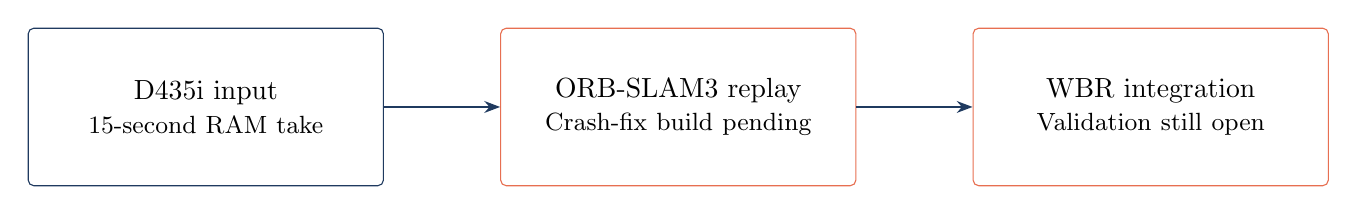
\begin{tikzpicture}[stage/.style={box,text width=43mm,minimum height=20mm,font=\normalsize}]
\node[stage] (a) at (0,0) {D435i input\\\small 15-second RAM take};
\node[stage,draw=fault] (b) at (6,0) {ORB-SLAM3 replay\\\small Crash-fix build pending};
\node[stage,draw=fault] (c) at (12,0) {WBR integration\\\small Validation still open};
\draw[flow] (a)--(b);\draw[flow] (b)--(c);
\end{tikzpicture}
\par\bigskip\raggedright
\deckitems{\item Three runs of EuRoC MH01, a dataset with a reference trajectory, measured 3.7--4.2 cm trajectory error; under-voltage invalidates their speed result.
\item The 8 GB Pi boots, but supply, large-data storage and D435i calibration are unresolved.
\item STM32H7 retains body estimation, balance, motor and jump safety.}
\vfill\takeaway{First deployment: optional position information during supervised slow motion.}
\src{experiments/2026-10-13-SESSION_FACTS_FOR_SLIDES.md; experiments/2026-10-14-SESSION_FACTS_ADDENDUM.md; experiments/2026-10-13-n4a-euroc-mh01/REPORT.md; docs/ARCHITECTURE.md}
\note{Historical observations only; no gate PASS. EuRoC ATE RMSE 0.0368--0.0416 m was on the former 4 GB board under under-voltage. Patch 4 was applied in an isolated copy; its rebuild and post-fix replay remain unverified. A 15 s memory-backed stereo take reported no drops. ATE means absolute trajectory error. Diagram is conceptual.}
\end{frame}

\begin{frame}{The whole road: today to a supervised robot trial}
\centering
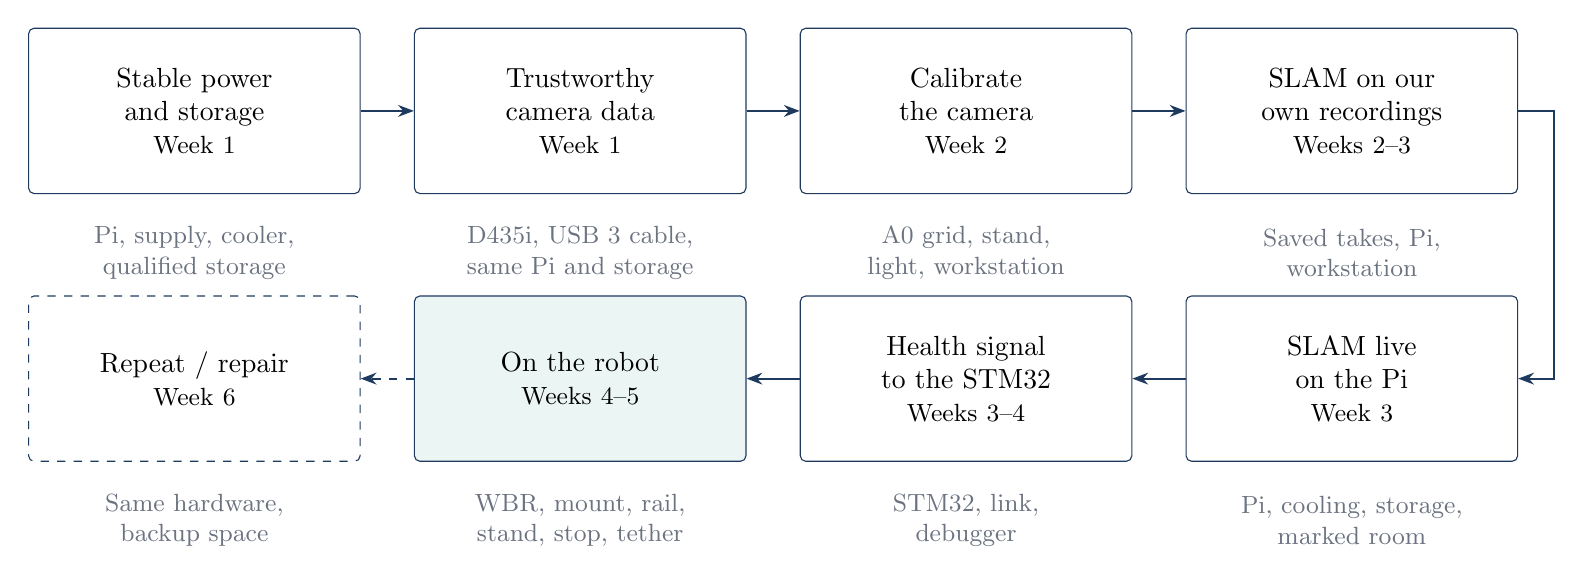
\begin{tikzpicture}[stage/.style={box,text width=40mm,minimum height=21mm,font=\normalsize},hw/.style={align=center,text width=40mm,font=\small,text=muted}]
\node[stage] (a) at (0,0) {Stable power\\and storage\\\small Week 1};
\node[stage] (b) at (4.9,0) {Trustworthy\\camera data\\\small Week 1};
\node[stage] (c) at (9.8,0) {Calibrate\\the camera\\\small Week 2};
\node[stage] (d) at (14.7,0) {SLAM on our\\own recordings\\\small Weeks 2--3};
\draw[flow](a)--(b);\draw[flow](b)--(c);\draw[flow](c)--(d);
\node[hw] at (0,-1.8) {Pi, supply, cooler,\\qualified storage};
\node[hw] at (4.9,-1.8) {D435i, USB 3 cable,\\same Pi and storage};
\node[hw] at (9.8,-1.8) {A0 grid, stand,\\light, workstation};
\node[hw] at (14.7,-1.8) {Saved takes, Pi,\\workstation};
\node[stage] (e) at (14.7,-3.4) {SLAM live\\on the Pi\\\small Week 3};
\node[stage] (f) at (9.8,-3.4) {Health signal\\to the STM32\\\small Weeks 3--4};
\node[stage,fill=teal!10] (g) at (4.9,-3.4) {On the robot\\\small Weeks 4--5};
\node[stage,dashed] (h) at (0,-3.4) {Repeat / repair\\\small Week 6};
\draw[flow](d.east)--++(.45,0)|-(e.east);
\draw[flow](e)--(f);\draw[flow](f)--(g);\draw[flow,dashed](g)--(h);
\node[hw] at (14.7,-5.2) {Pi, cooling, storage,\\marked room};
\node[hw] at (9.8,-5.2) {STM32, link,\\debugger};
\node[hw] at (4.9,-5.2) {WBR, mount, rail,\\stand, stop, tether};
\node[hw] at (0,-5.2) {Same hardware,\\backup space};
\end{tikzpicture}
\par\medskip\raggedright\small Conditional weeks from 14 October. A failed step moves the schedule; it never shortens a test.
\src{slides_roadmap/ROADMAP.md; slides_roadmap/research/R3_plan.md}
\note{Existing gates in order: preparation; N0--N3; N4A/N4B; N4C/N5; N6; N7 supported then separately authorized motion. N6 design may overlap after controller review; acceptance follows N5. Optional navigation is after this route.}
\end{frame}

\begin{frame}{A few terms make the plan easier to read}
\small\renewcommand{\arraystretch}{1.18}
\begin{tabular}{@{}L{42mm}L{142mm}@{}}\toprule
\textbf{Term} & \textbf{Meaning in this roadmap}\\\midrule
SLAM & Simultaneous localization and mapping: estimate camera position while building a map.\\
VIO / IMU & Visual-inertial odometry combines images with an inertial measurement unit: gyroscope and accelerometer.\\
Calibration & Measure camera geometry, camera--IMU alignment, timing offset and sensor noise.\\
ROS / bag / replay & Robot Operating System passes messages; a bag records them; replay feeds a saved recording back into software.\\
Pose / frame / reset & Pose is position and orientation; frame defines axes and origin; reset starts a new estimate.\\
Health / optional input & Health reports valid, lost or old estimates. Optional position information never owns balance or motor safety.\\\bottomrule\end{tabular}
\src{docs/ARCHITECTURE.md; docs/DECISIONS.md; slides_roadmap/ROADMAP.md}
\note{Planning proposal only; bookings, hardware availability and acceptance remain unconfirmed.}
\end{frame}

\begin{frame}{Stable power and storage}
\relax
{\small\color{muted}Preparation; platform check N0}\par\medskip
\phase{Make the next lab visit usable.}
{Confirm parts, qualify the data path, prepare the target and prove file conversion on synthetic data.}
{Power/storage checks; offline image and IMU conversion; checksums for exact-copy verification.}
{8 GB Pi, 5.1 V/5 A supply, cooler, storage, local console; camera stays idle.}
{Named owners for every blocker; conversion preserves pixels, counts, units and timestamps on known samples.}
{2--5 engineer-days; parts and workstation waits are additional.}
\src{experiments/2026-10-14-SESSION_FACTS_ADDENDUM.md; experiments/2026-09-12-pi5-native-sensor-validation/N3_PREPARATION.md; docs/D435I_CALIBRATION_PLAN.md}
\note{The 8 GB Pi booted the existing 32 GB card, but under-voltage persists. Current SDK package is 2.58.4. Candidate RealSense ROS 4.58.4/messages were inspected, not installed. A 64 GB USB 2 stick measured 1.09 MB/s. User's microSD exception covers calibration/VIO only; large N3 bags need separately qualified storage. The current D435i SDK serial is 317422076650; ASIC and separately observed USB descriptor are 327743061057. Firmware-update ID remains independently unverified. Do not reuse the old SDK serial from the N3 preparation note. Kalibr's primary tools require ROS 1 bag data; .db3 is rosbag2. The chosen PNG/CSV conversion is a future reviewed utility.}
\end{frame}

\begin{frame}{Resolve these dependencies before camera time}
\small\renewcommand{\arraystretch}{1.18}
\begin{tabular}{@{}L{34mm}L{72mm}L{78mm}@{}}\toprule
\textbf{Dependency} & \textbf{Current state} & \textbf{Next owner action}\\\midrule
Power / access & 5 V/3 A still under-voltages; ordered supply arrival unknown. Wi-Fi unverified; Ethernet loose. & Confirm suitable supply/cooling and local console or verified network access.\\
ROS / storage & Camera wrapper not installed. USB stick measured 1.09 MB/s. & Review installation separately; borrow or buy and qualify large-bag storage.\\
Calibration tools & ROS 1 bag conversion and long stationary recorder are untested. & Prove conversion offline; confirm workstation and recorder stop/recovery.\\
Target / people & Measured target, overnight permission and controller owner unconfirmed. & Prepare print; name controller engineer; request conditional lab slots.\\\bottomrule\end{tabular}\vfill\takeaway{The owner must explicitly authorize camera work before any capture.}
\src{experiments/2026-10-14-SESSION_FACTS_ADDENDUM.md; experiments/2026-09-12-pi5-native-sensor-validation/N3_PREPARATION.md; docs/D435I_CALIBRATION_PLAN.md}
\note{The 8 GB Pi booted the existing 32 GB card, but under-voltage persists. Current SDK package is 2.58.4. Candidate RealSense ROS 4.58.4/messages were inspected, not installed. A 64 GB USB 2 stick measured 1.09 MB/s. User's microSD exception covers calibration/VIO only; large N3 bags need separately qualified storage. The current D435i SDK serial is 317422076650; ASIC and separately observed USB descriptor are 327743061057. Firmware-update ID remains independently unverified. Do not reuse the old SDK serial from the N3 preparation note. Kalibr's primary tools require ROS 1 bag data; .db3 is rosbag2. The chosen PNG/CSV conversion is a future reviewed utility.}
\end{frame}

\begin{frame}{Trustworthy camera data}
\relax
{\small\color{muted}Input checks N0 $\to$ N1 $\to$ N2 $\to$ N3}\par\medskip
\phase{Prove the same camera can stream, record and replay reliably.}
{Check platform, USB and raw data in order; then record ROS messages and compare full replay.}
{Guarded sensor checks; reviewed ROS 2 Jazzy camera driver; recording/replay comparison.}
{Same Pi, stable supply/cooler, D435i, direct USB 3 cable and qualified bag storage.}
{USB reports at least 5000M; all three raw tests meet the next page; recorded and replayed counts/fields agree.}
{0.5--3 engineer-days; reserve 3--4 h, with diagnosis allowed to use the slot.}
\src{experiments/2026-09-12-pi5-native-sensor-validation/PHASE_A_RUNBOOK.md; experiments/2026-10-14-lab-prep/LAB_RUNBOOK_2026-10-15.md}
\note{N2 exact profile: IR1 Y8 640x480/15, gyro/200, accel/100. Rate bands: 14.25--15.75, 190--210 and 95--105 Hz; image gaps <=0.20 s, motion gaps <=0.05 s; timestamps/frame steps positive and no image frames missing. Retain all startup, boundary, content, kernel, power, health and normal-stop checks. N3 contains required image/CameraInfo/raw gyro/raw accel/IMUInfo/extrinsics/TF topics, QoS context and complete decoded replay comparison. Diagnostic latched power never promotes PASS or enters N3. No camera-dependent action before explicit owner authorization.}
\end{frame}

\begin{frame}{What a trustworthy raw recording looks like}
\relax
{\small\color{muted}Raw-data check N2; ROS record/replay N3 follows}\par\medskip\small\renewcommand{\arraystretch}{1.18}
\begin{tabular}{@{}L{47mm}L{137mm}@{}}\toprule
\textbf{Check} & \textbf{Required visible result}\\\midrule
Exact raw profile & IR1: Y8 grayscale, 640×480 at 15 Hz; gyroscope 200 Hz; accelerometer 100 Hz.\\
Three stages & 20 seconds, then 105 seconds, then the mandatory 300-second soak.\\
Measured rates & Image 14.25--15.75 Hz; gyro 190--210 Hz; accel 95--105 Hz.\\
Gaps and order & Image gaps ≤0.20 s; motion gaps ≤0.05 s; increasing timestamps/frame numbers; no missing image frames.\\
Health and stop & All original startup, boundary, content, kernel, power and normal-stop checks reviewed; raw logs retained.\\\bottomrule\end{tabular}\vfill\takeaway{A short successful take does not replace the five-minute soak.}
\src{experiments/2026-09-12-pi5-native-sensor-validation/PHASE_A_RUNBOOK.md; experiments/2026-10-14-lab-prep/LAB_RUNBOOK_2026-10-15.md}
\note{N2 exact profile: IR1 Y8 640x480/15, gyro/200, accel/100. Rate bands: 14.25--15.75, 190--210 and 95--105 Hz; image gaps <=0.20 s, motion gaps <=0.05 s; timestamps/frame steps positive and no image frames missing. Retain all startup, boundary, content, kernel, power, health and normal-stop checks. N3 contains required image/CameraInfo/raw gyro/raw accel/IMUInfo/extrinsics/TF topics, QoS context and complete decoded replay comparison. Diagnostic latched power never promotes PASS or enters N3. No camera-dependent action before explicit owner authorization.}
\end{frame}

\begin{frame}{Calibrate the camera: collect usable measurements}
\relax
{\small\color{muted}Calibration acquisition within N4A / N4B}\par\medskip
\phase{Measure this unit rather than rely on example defaults.}
{Record three target-motion takes; separate room trials and stationary noise data; inspect the first take.}
{Reviewed stereo recorder; future long-duration IMU recorder; verified lossless export.}
{Same camera/Pi, measured A0 AprilGrid (tag-pattern target), stand, light, calipers and backup space.}
{Three 120 s target takes and separate 90 s room trials have usable images and ordered timing; two copies match.}
{1--2 engineer-days; 3--4 h target slot; separately 30 min warm-up + 15--24 h stationary data.}
\src{docs/D435I_CALIBRATION_PLAN.md; slides_roadmap/research/R3_plan.md; https://github.com/ethz-asl/kalibr/wiki/camera-imu-calibration; https://github.com/ethz-asl/kalibr/wiki/IMU-Noise-Model}
\note{After N0--N3, separately attest IR1+IR2 Y8 640x480/30, gyro/200, accel/100, emitter OFF. S=120 s; C1--C3=120 s each; six-pose I diagnostics; V1--V3=90 s. Target: measured 6x6 AprilGrid, 80 mm tags, spacing ratio 0.25; 580 mm pattern, >=740 mm with one-tag border, A0. Warm camera 30 min. The existing four-stream recorder is limited to 120 s. Kalibr recommends stationary 15--24 h; this is not a mandatory gate duration. Fixed target, low blur and all-axis excitation are required. Never run stationary and moving-target captures together.}
\end{frame}

\begin{frame}{SLAM on our own recordings}
\relax
{\small\color{muted}Known reference N4A; camera replay N4B}\par\medskip
\phase{Check repeatable output before going live.}
{Finish the existing crash-fix build; rerun the known EuRoC dataset; calibrate and replay three own-camera takes plus unused evaluation data.}
{Native ORB-SLAM3; Kalibr alignment/timing solver; Allan noise analysis; trajectory plots.}
{8 GB Pi with stable power; confirmed ROS 1/Kalibr workstation; immutable saved takes.}
{Build loads; three replay results show initialization, tracking losses and resets; settings and calibration have traceable reports.}
{2--4 engineer-days; add 2--5 days if import/tool compatibility fails.}
\src{experiments/2026-10-14-SESSION_FACTS_ADDENDUM.md; docs/D435I_CALIBRATION_PLAN.md; https://github.com/ethz-asl/kalibr/wiki/bag-format; https://github.com/ethz-asl/kalibr/wiki/yaml-formats}
\note{Previous EuRoC MH01 accuracy is known-input evidence only; rerun on the target Pi after stable power before timing claims. Existing patch-4 rebuild was interrupted. Kalibr expects ROS 1 bags; chosen proposal is lossless PNG and full-precision timestamped IMU CSV followed by Kalibr bagcreater, after synthetic/known-sample verification. RealSense .db3 is ROS 2 rosbag2 and must not be assumed readable. Kalibr T_cam_imu is IMU-to-camera; invert for the ORB camera-to-IMU input. Apply t_imu=t_cam+shift once before association, preserve raw stamps. Calibration thresholds are proposed and need review. Keep all failed runs and the original calibration warning.}
\end{frame}

\begin{frame}{SLAM live on the Pi}
\relax
{\small\color{muted}Live estimator N4C; sustained resources N5}\par\medskip
\phase{See whether current camera position arrives in time.}
{Hold settings fixed; run three repeats and a proposed 30-minute load with growing map, revisits and recovery.}
{ORB without a display; estimate-age, queue, drop/reset, processor/memory, temperature and power plots.}
{Final Pi/camera/cooling/data path, textured marked route, operator and reviewer.}
{Full logs account for inputs and outputs; queues do not grow; age/resource plots stay within limits approved before testing.}
{1--3 engineer-days; book 2--3 h after recorded-data review.}
\src{slides_roadmap/research/R1_algorithms.md section 5; slides_roadmap/research/R2_integration.md; slides_course/main.tex N4C/N5}
\note{Measure capture-to-pose only with validated clock mapping and uncertainty. Otherwise age is unknown. Report P50/P95/P99 for age, waiting, tracking and publish separately; count input/output/drop/reset events. Candidate age, CPU and thermal values in earlier research are screening scenarios only, not safety limits. The controller owner ratifies acceptance limits before N6 or motor tests. A 33.3 ms period for 30 Hz is arithmetic, not a Pi speed guarantee. Offline replay is not live throughput.}
\end{frame}

\begin{frame}{Measure how old an estimate is}
\deckitems{
\item Estimate age is the time from image capture to the position result being available.
\item First prove how camera and Pi clocks relate. If that relation is unknown, age is unknown.
\item Report the median and the 95th/99th percentiles: values below which 50/95/99\% of samples fall.
\item Count every missing input, queued frame, tracking loss and reset alongside CPU, memory, heat and power.
}
\vfill\takeaway{A fresh status message cannot make an old camera estimate fresh.}
\src{slides_roadmap/research/R1_algorithms.md section 5; slides_roadmap/research/R2_integration.md; slides_course/main.tex N4C/N5}
\note{Measure capture-to-pose only with validated clock mapping and uncertainty. Otherwise age is unknown. Report P50/P95/P99 for age, waiting, tracking and publish separately; count input/output/drop/reset events. Candidate age, CPU and thermal values in earlier research are screening scenarios only, not safety limits. The controller owner ratifies acceptance limits before N6 or motor tests. A 33.3 ms period for 30 Hz is arithmetic, not a Pi speed guarantee. Offline replay is not live throughput.}
\end{frame}

\begin{frame}{Algorithm comparison: keep one default, test one challenger}
\small Scores from the independent review, checked against the algorithm review; judgments, not Pi benchmarks.\par\smallskip\small\linespread{1.03}\selectfont\renewcommand{\arraystretch}{1.05}
\begin{tabular}{@{}L{58mm}L{13mm}L{12mm}L{17mm}L{13mm}L{61mm}@{}}\toprule
\textbf{Candidate} & \textbf{Demo} & \textbf{CPU} & \textbf{Motion} & \textbf{/100} & \textbf{Decision}\\\midrule
ORB-SLAM3 stereo/IMU & 5 & 3 & 3 & 68 & Default; existing tools\\
RTAB-Map own motion estimate & 3 & 2 & 3 & 68 & For an obstacle map\\
OpenVINS & 3 & 4 & 3 & 61 & First matched-data challenger\\
Wheels/body + depth & 2 & 5 & 2 & 56 & Requires working robot exports\\
ORB RGB-D & 3 & 3 & 2 & 52 & New input path needed\\
Basalt & 2 & 3 & 3 & 53 & Prove build/adapter benefit\\
VINS-Fusion & 2 & 3 & 3 & 47 & Prove port benefit\\
Kimera-VIO & 2 & 2 & 3 & 48 & More dependencies; defer\\\bottomrule\end{tabular}\par\smallskip\small 1--5: higher = better fit. RGB-D = color + depth. Total weights: demo 30\%, CPU 20\%, motion 20\%, software support 15\%, navigation 10\%, licence 5\%.
\src{slides_roadmap/research/R1_algorithms.md; slides_roadmap/research/R1b_algorithms_independent.md}
\note{Exact R1b components D,C,R,J,N,L: ORB 5,3,3,2,3,2=68; RTAB own 3,2,3,5,5,5=68; OpenVINS 3,4,3,3,2,2=61; no SLAM 2,5,2,3,2,3=56; RGB-D 3,3,2,2,3,2=52; Basalt 2,3,3,2,3,5=53; VINS 2,3,3,1,3,2=47; Kimera 2,2,3,1,4,5=48. Total = (30D+20C+20R+15J+10N+5L)/5. RTAB external odometry 54 is a later composition, not a second local estimator. DROID/DPVO class 36 fails the CPU-only deployment constraint. Research snapshot, not new benchmarks.}
\end{frame}

\begin{frame}{What would make us change the algorithm?}
\deckitems{
\item Keep ORB-SLAM3 for the first position-estimation trial: build and input work already exist, but live Pi performance is still open.
\item If trusted data and correct calibration still miss approved age or continuity limits, spend at most 2--3 days diagnosing; compare OpenVINS on identical retained recordings.
\item Switch only if the challenger meets the same approved limits and its build, input conversion and failure behavior are verified.
\item If the first goal becomes an obstacle/occupancy map, compare RTAB-Map under the complete Pi workload.
\item A demonstrated wheel/body interface could make a smaller rolling demo faster; it changes the deliverable and does not prove camera VIO.
}
\src{slides_roadmap/research/R1_algorithms.md; slides_roadmap/research/R1b_algorithms_independent.md; https://github.com/UZ-SLAMLab/ORB_SLAM3; https://github.com/rpng/open_vins/pull/500; https://github.com/introlab/rtabmap_ros/tree/ros2}
\note{Algorithm scores on the preceding page are judgment-based, not measured Pi/WBR results. OpenVINS Jazzy pull request 500 remains open at this snapshot; budget port/build work. RTAB-Map is a mapping-first alternative, not the selected first estimator. Wheel/body plus depth changes the deliverable and does not qualify VIO.}
\end{frame}

\begin{frame}{Health signal to the STM32}
\relax
{\small\color{muted}Receiver review and acceptance N6}\par\medskip
\phase{Tell the controller when optional position information is usable.}
{Review the link, clocks, axes and invalidation rules; test missing, frozen, reset and corrupt input on synthetic cases.}
{Proposed bounded receiver; expected-versus-actual traces; local timeout on the STM32.}
{Named controller engineer, confirmed STM32H7 board, reviewed link and debugger.}
{Traces show old/wrong/corrupt input rejected and optional input withdrawn after Pi/link loss within approved limits.}
{2--4 engineer-days; design may overlap after review; acceptance follows sustained Pi tests.}
\src{docs/ARCHITECTURE.md; docs/DECISIONS.md; slides_roadmap/research/R2_integration.md sections 1,2}
\note{N6 acceptance follows N5. Design/fixtures may be prepared earlier only after the controller owner reviews the proposal. No API, message, transport or firmware is implemented or accepted here. Validate finite values, CRC/length/version, sequence/session/time wraps, clock mapping uncertainty, wrong frames, stale/frozen source, reset/map jump and Pi/link loss. Fresh heartbeat cannot refresh old source time. Invalid input cannot renew a lease. Controller retains balance and motor/jump safety. Do not invent fixed rates/timeouts.}
\end{frame}

\begin{frame}{On the robot: mounting and supported tests}
\relax
{\small\color{muted}Supported integration N7}\par\medskip
\phase{Verify power, mounting and controller independence.}
{Review mount/axes and power rail; test with motors disabled, then separately approved supported faults.}
{Reviewed receiver; power, controller-loop and estimate-age traces; controlled fault tests.}
{WBR, controller owner, battery/converter/fuse/link, mount/cooler, rated stand and independent stop.}
{Logs show no unexpected actuation/reset or control-loop violation; each fault removes optional input within approved limits.}
{1--3 engineer-days; book 3--4 h after receiver review.}
\src{slides_roadmap/research/R2_integration.md sections 3,5; slides_roadmap/research/R3_plan.md; https://www.raspberrypi.com/documentation/computers/raspberry-pi.html}
\note{Review battery and DC-DC under worst approved motor load, USB power, heat, EMI/grounding and independent controller supply. Record rigid torso transform, cable strain relief, view through allowed pitch/leg travel and payload/center-of-mass change. Refresh USB/profile/calibration checks after topology changes. Static stereo-inertial may remain uninitialized. Do not start a motor test without separately reviewed safety sequence and controller owner.}
\end{frame}

\begin{frame}{On the robot: supervised slow motion}
\relax
{\small\color{muted}Separately authorized motion N7}\par\medskip
\phase{Repeat a slow trial while local balance remains independent.}
{Baseline the controller; use approved tethered trials and bounded manual room motion; test Pi loss and repeat startup/stop.}
{Operator runbook; checksummed utility bundle; Pi and STM32 traces.}
{Approved tether/cleared route, local stop, controller owner, operator and spotter.}
{Retained trials meet agreed motion/stop limits; Pi loss is handled; another operator reproduces startup, stop and rollback.}
{1--4 engineer-days; 2--3 h motion plus a separate repeat/repair slot.}
\src{slides_roadmap/research/R2_integration.md section 5; slides_roadmap/research/R3_plan.md; AGENTS.md}
\note{Physical motion requires separate approval. Predeclare speed/turn/acceleration, stopping, clearance, repeat count and pass/fail bounds. Controller selects balance-preserving bounded stop policy; never blindly remove torque on Pi loss. Keep reset recovery operator-controlled. Without synchronized reference, report return/checkpoint as proxy, not room ATE. State tether loading. No jump/fall survivability claim.}
\end{frame}

\begin{frame}{Hardware and lab bookings: bench and calibration}
\small\linespread{1.03}\selectfont\renewcommand{\arraystretch}{1.05}
\begin{tabular}{@{}L{40mm}L{29mm}L{31mm}L{32mm}L{46mm}@{}}\toprule
\textbf{Item} & \textbf{Phase} & \textbf{Status} & \textbf{Book when} & \textbf{Prepare first}\\\midrule
8 GB Pi + D435i & Input $\to$ live & Have per notes; confirm loan & W1; retain through W6 & Same unit, console, USB 3 cable\\
5.1 V/5 A supply + cooler & All Pi work & Supply ordered; cooler confirm with lab & Before first camera slot & Confirm arrival and power checks\\
Large-data storage & Input $\to$ live & Borrow / buy; unqualified & Before W1 input slot & Sustained-write and replay checks\\
128 GB microSD & Calibration only & Ordered; arrival unknown & Before target slot & Confirm exception; qualify short takes\\
A0 grid, stand, light, calipers & Calibration & Print/buy; tools confirm with lab & W2: 3--4 h & Measure grid, prove import route\\
Quiet bench + workstation & Calibration & Lab; confirm access & W2: 30 min + 15--24 h & Test IMU recorder, backup and stop\\\bottomrule\end{tabular}
\src{slides_roadmap/ROADMAP.md; slides_roadmap/research/R3_plan.md}
\note{No inventory or reservation verified by this task. Slow 64 GB USB 2 stick is not qualified large-data storage. Card exception is calibration/VIO-only. Acquire locally on Pi. Target: 6x6, 80 mm tags, spacing 0.25; measured A0 with rigid backing.}
\end{frame}

\begin{frame}{Hardware and lab bookings: live Pi and robot}
\small\linespread{1.03}\selectfont\renewcommand{\arraystretch}{1.05}
\begin{tabular}{@{}L{40mm}L{29mm}L{31mm}L{32mm}L{46mm}@{}}\toprule
\textbf{Item} & \textbf{Phase} & \textbf{Status} & \textbf{Book when} & \textbf{Prepare first}\\\midrule
Marked textured room & Live Pi & Lab; confirm route & W3: 2--3 h & Replay accepted; age/resource limits\\
STM32H7 + link + debugger & Health signal & Lab; board/owner unknown & W3--4; after review & Confirm board, voltage, pins and link\\
WBR + mount + battery rail & Supported robot & Lab; stock/design unknown & W4: 3--4 h & Review mount/power; receiver tests\\
Rated stand + independent stop & Supported robot & Lab; confirm suitability & With controller owner in W4 & Approve fault procedure\\
Tether + clear route + spotter & Slow robot motion & Lab; confirm suitability & W5: 2--3 h & Supported tests; separate motion approval\\
Repeat/repair access + backups & Handoff & Lab; confirm access & W6: 2--4 h reserve & Preserve failures; list unresolved work\\\bottomrule\end{tabular}
\src{slides_roadmap/ROADMAP.md; slides_roadmap/research/R3_plan.md}
\note{Planning proposal only; bookings, hardware availability and acceptance remain unconfirmed.}
\end{frame}

\begin{frame}{Software stack by phase}
\small\linespread{1.03}\selectfont\renewcommand{\arraystretch}{1.05}
\begin{tabular}{@{}L{40mm}L{86mm}L{58mm}@{}}\toprule
\textbf{Phase} & \textbf{Software / purpose} & \textbf{What must be ready}\\\midrule
Preparation / input & Ubuntu + ROS 2 Jazzy; RealSense SDK/driver; existing raw checks; rosbag2 recorder/replay. & Review wrapper install; verify actual profiles and complete replay.\\
Calibration & Lossless PNG + full-precision IMU export $\to$ ROS 1 bag; Kalibr; Allan sensor-noise analysis. & Conversion/workstation and long recorder are future reviewed tools.\\
Saved-data / live SLAM & Native ORB-SLAM3 stereo-inertial; existing adapter; trajectory and health/resource plots. & Finish existing fix; preserve versions, settings and raw evidence.\\
STM32 health & Small reviewed Pi health adapter + bounded STM32 receiver; synthetic rejection tests. & Message, link and limits need controller approval before implementation.\\
Robot / handoff & Same frozen stack; startup/stop/rollback runbook; checksummed runtime bundle. & No balance authority on Pi; reuse a validated controller link.\\\bottomrule\end{tabular}\par\smallskip\small Defer extra ports, Pi graphics and navigation until needed.
\src{slides_roadmap/ROADMAP.md; slides_roadmap/research/R3_plan.md}
\note{Planning proposal only; bookings, hardware availability and acceptance remain unconfirmed.}
\end{frame}

\begin{frame}{Next six weeks: preparation through live Pi}
\small\renewcommand{\arraystretch}{1.18}
\begin{tabular}{@{}L{27mm}L{48mm}L{61mm}L{48mm}@{}}\toprule
\textbf{Week} & \textbf{Owner / lab} & \textbf{Engineering work} & \textbf{Visible result}\\\midrule
1: 14--20 Oct & Confirm parts, camera loan, storage, console and workstation; request 3--4 h bench. & Prove conversion offline; target/recorder preparation; fresh input checks after authorization. & Reviewed input/replay receipts or a precise blocker.\\
2: 21--27 Oct & Book target 3--4 h and separate overnight; same camera/Pi. & Three target takes, unused room takes, stationary data; first-take review and backups. & Usable captures, two matching copies; calibration reports or recapture decision.\\
3: 28 Oct--3 Nov & Workstation; reserve marked route 2--3 h; agree controller limits. & Stable-power reference; repeated own-data replay; live and sustained-load measurements. & Tracking/reset and estimate-age plots; no growing queue; accept or diagnose.\\\bottomrule\end{tabular}\par\medskip\small Dates are conditional targets. Unmet prerequisites carry forward; the soak and overnight recording remain unchanged.
\src{slides_roadmap/ROADMAP.md; slides_roadmap/research/R3_plan.md}
\note{Planning proposal only; bookings, hardware availability and acceptance remain unconfirmed.}
\end{frame}

\begin{frame}{Next six weeks: controller, robot and contingency}
\small\renewcommand{\arraystretch}{1.18}
\begin{tabular}{@{}L{27mm}L{48mm}L{61mm}L{48mm}@{}}\toprule
\textbf{Week} & \textbf{Owner / lab} & \textbf{Engineering work} & \textbf{Visible result}\\\midrule
4: 4--10 Nov & Controller owner; confirmed WBR, board, link, stand and stop; 3--4 h. & Accept receiver after live/resource review; motors-disabled then approved supported faults; mount/power checks. & Rejection/fallback traces and unchanged local control within approved limits.\\
5: 11--17 Nov & Separate motion approval; tether, route, operator/spotter; 2--3 h. & Supervised slow motion, Pi-loss trial, repeat startup/stop and review vibration/age. & Target: mounted tracking plus verified health/fallback behavior; no navigation claim.\\
6: 18--24 Nov & Hold 2--4 h repair/repeat slot; extend camera loan if needed. & Resolve the failing layer; freeze utility/settings bundle; second-operator repeat. & Reproduction report, verified backups and explicit remaining blockers.\\\bottomrule\end{tabular}\vfill\takeaway{If week 4 slips, finish supported tests before moving the robot.}
\src{slides_roadmap/ROADMAP.md; slides_roadmap/research/R3_plan.md}
\note{Planning proposal only; bookings, hardware availability and acceptance remain unconfirmed.}
\end{frame}

\begin{frame}{Navigation is a later project.}
\centering
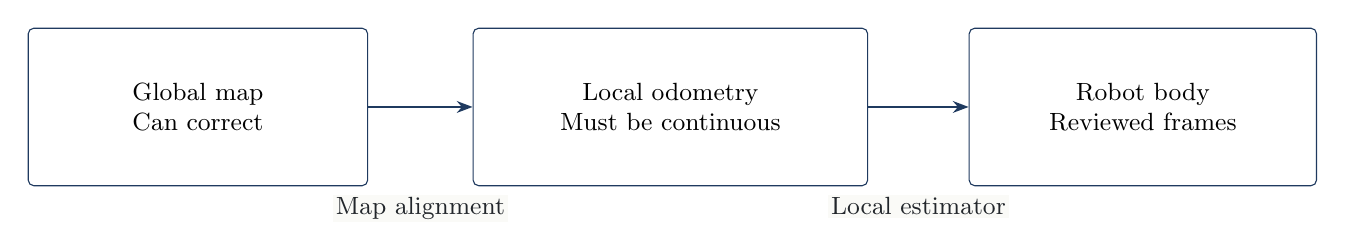
\begin{tikzpicture}[font=\normalsize]
\node[box,text width=41mm,minimum height=20mm] (m) at (0,0) {Global map\\Can correct};
\node[box,text width=48mm,minimum height=20mm] (o) at (6,0) {Local odometry\\Must be continuous};
\node[box,text width=42mm,minimum height=20mm] (b) at (12,0) {Robot body\\Reviewed frames};
\draw[flow](m)--node[below=11mm,lbl]{Map alignment}(o);
\draw[flow](o)--node[below=11mm,lbl]{Local estimator}(b);
\end{tikzpicture}
\par\medskip
\deckitems{\item Validate acquisition-stamped wheel/body/contact telemetry, geometry, clocks and slip before fusion.
\item Qualify obstacle coverage and occupancy mapping; sparse ORB landmarks are not an obstacle map.
\item Nav2, a ROS navigation stack, needs reviewed continuous odometry, frames, stop bounds and controller veto.}
\par\medskip\small D435i depth is a candidate obstacle sensor, not a qualified input.
\src{https://github.com/ros-infrastructure/rep/blob/master/rep-0105.rst; https://docs.nav2.org/jazzy/configuration_and_development/first_time_robot_setup_guide/odom/setup_robot_localization/; https://github.com/introlab/rtabmap_ros/tree/ros2}
\note{Optional post-N7 objective. Diagram is conceptual, not an approved coordinate-frame graph. Global map correction must not jump the local motion state. Keep camera/body IMUs separate and avoid double-counting camera IMU or correlated wheel measurements.}
\end{frame}

\begin{frame}{The route traces to project evidence and primary sources.}
\small\deckitems{
\item \textbf{Project state:} 13--14 October facts, N3 preparation, current lab runbook, calibration plan and N4A report.
\item \href{https://github.com/ethz-asl/kalibr/wiki/bag-format}{\textbf{Kalibr bag format}} and \href{https://github.com/ethz-asl/kalibr/wiki/ROS2-Calibration-Using-Kalibr}{recording conversion}; \href{https://github.com/ethz-asl/kalibr/wiki/IMU-Noise-Model}{noise guidance}.
\item \href{https://github.com/realsenseai/librealsense/blob/master/doc/record-and-playback.md}{\textbf{RealSense .db3 recording}} uses ROS 2 rosbag2 format.
\item \href{https://www.raspberrypi.com/documentation/computers/raspberry-pi.html}{\textbf{Raspberry Pi power guidance}} and \href{https://www.raspberrypi.com/products/27w-power-supply/}{official supply specification}.
\item \href{https://github.com/gjcliff/ORB_SLAM3_ROS2}{\textbf{Current cited ORB ROS wrapper}} and \href{https://github.com/rpng/open_vins/pull/500}{OpenVINS Jazzy proposal}.
\item \href{https://github.com/ros-infrastructure/rep/blob/master/rep-0105.rst}{\textbf{REP-105}}, \href{https://docs.nav2.org/jazzy/configuration_and_development/first_time_robot_setup_guide/odom/setup_robot_localization/}{Nav2 Jazzy odometry} and \href{https://github.com/introlab/rtabmap_ros/tree/ros2}{RTAB-Map mapping}.
}
\par\medskip\normalsize Durations, later acceptance limits and switch rules are planning proposals. Hardware, calibration, estimate age and deployed performance remain unverified.
\src{slides_roadmap/REVIEW.md; slides_roadmap/ROADMAP.md; slides_roadmap/research/R1_algorithms.md; slides_roadmap/research/R1b_algorithms_independent.md; slides_roadmap/research/R2_integration.md; slides_roadmap/research/R3_plan.md}
\note{External claims linked to primary upstream documentation. OpenVINS PR was open at the 14 October 2026 snapshot. Mutable repositories must be pinned before implementation. No hardware/process tests or gate acceptance occurred.}
\end{frame}
\end{document}
